\section{BATDONGSAN (PROPERTYGURU)}
\subsection{Giới thiệu}
\hspace*{1cm}Được ra mắt vào năm 2008, trang web Batdongsan.com.vn là một nền tảng hàng đầu tại Việt Nam trong lĩnh vực bất động sản. Với sứ mệnh cung cấp thông tin đầy đủ, chính xác và đa dạng về thị trường nhà đất. Năm 2010, trang web đã trở thành website hàng đầu trong lĩnh vực bất động sản. Vào tháng 10 năm 2018, sau khi chính thức gia nhập tập đoàn PropertyGuru,  PropertyGuru, Batdongsan.com.vn đã vươn lên một cách vượt trội nhờ tận dụng không ngừng lợi thế về công nghệ và dữ liệu từ tập đoàn lớn, từ đó trang web đã thực hiện nhiều cải tiến quan trọng như nâng cấp giao diện, cải thiện tính năng tìm kiếm và tăng tốc độ trải nghiệm. \cite{batdongsan} Batdongsan.com.vn không chỉ là nguồn tin tin cậy cho người mua và người bán mà còn là điểm đến đáng tin cậy cho những ai quan tâm đến thị trường bất động sản.\\
\hspace*{1cm}Batdongsan.com.vn cung cấp một loạt các danh mục bất động sản, từ căn hộ, nhà phố đến đất đai và dự án mới. Người dùng có thể dễ dàng tìm kiếm, so sánh và lựa chọn bất động sản phù hợp với nhu cầu và ước mơ của mình. Điều này giúp tối ưu hóa trải nghiệm người dùng và tiết kiệm thời gian trong quá trình tìm kiếm. Trang web không ngừng cập nhật thông tin về thị trường bất động sản, giúp người dùng có cái nhìn toàn diện về xu hướng giá cả, quy hoạch đô thị, và những dự án nổi bật. Điều này giúp người dùng đưa ra quyết định thông tin và hiệu quả. Ngoài việc cung cấp thông tin, Batdongsan.com.vn còn tạo ra một cộng đồng sôi động, nơi mà người dùng có thể chia sẻ kinh nghiệm, đánh giá về các dự án, và hỗ trợ nhau trong quá trình mua bán bất động sản. Điều này làm cho trang web trở thành điểm đến toàn diện cho mọi người quan tâm đến thị trường bất động sản tại Việt Nam.
\begin{figure}[H]
    \centering
    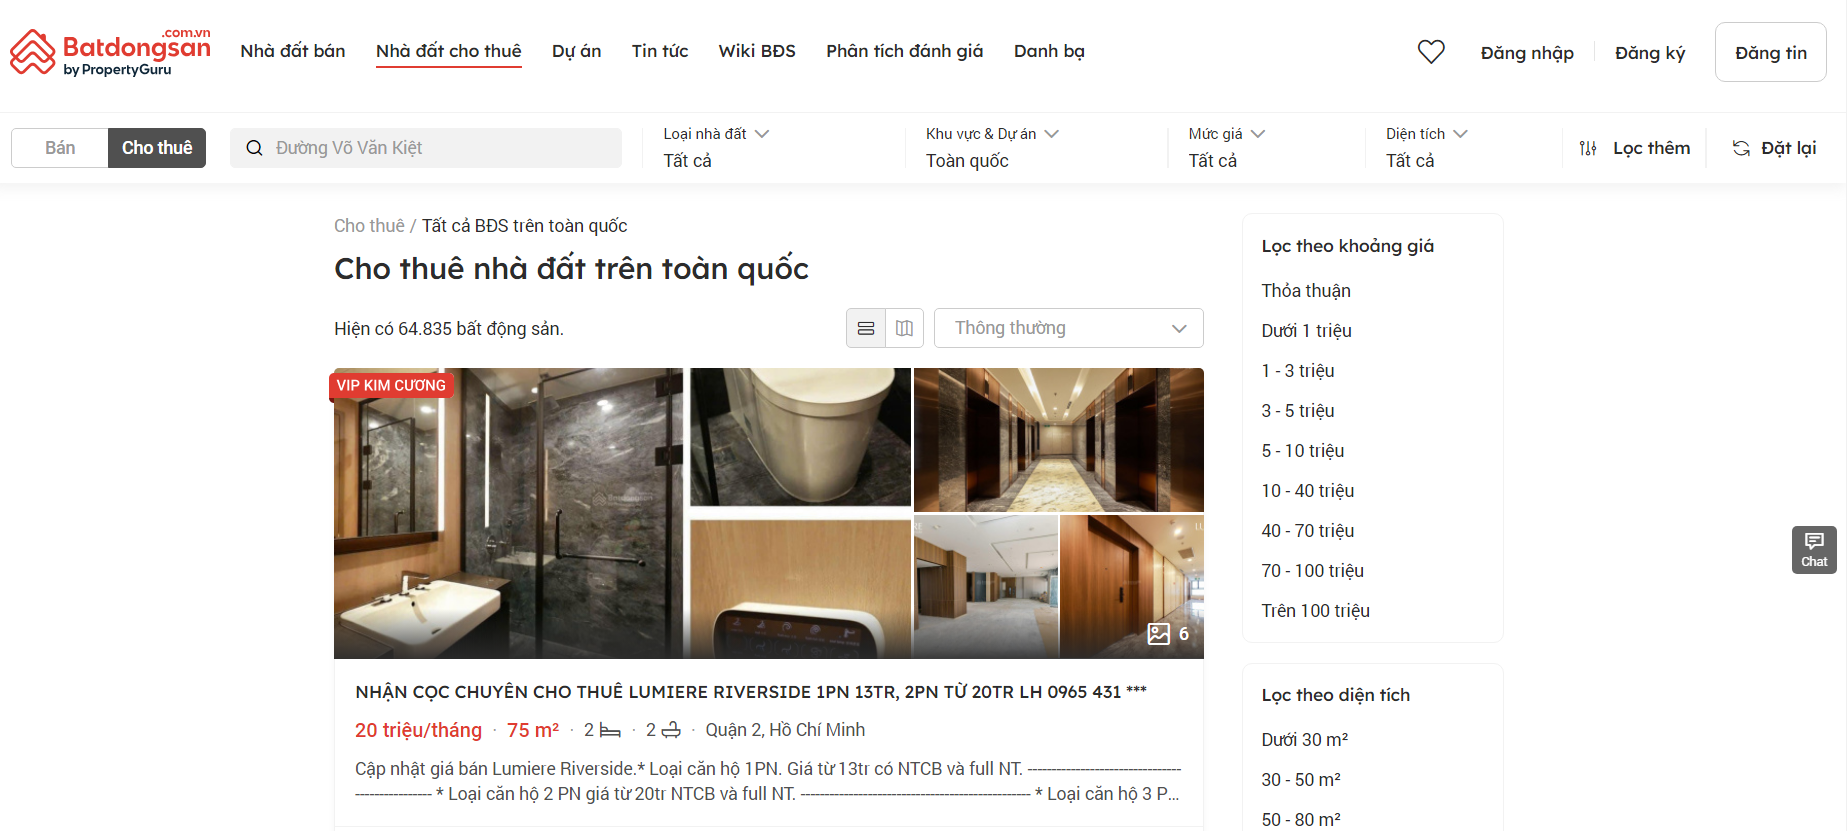
\includegraphics[width=1\textwidth]{Images/RelatedSystems/BatdongsanDesktop.png}
    \caption{Giao diện Batdongsan.com.vn trên website}
\end{figure}
\begin{figure}[H]
    \centering
    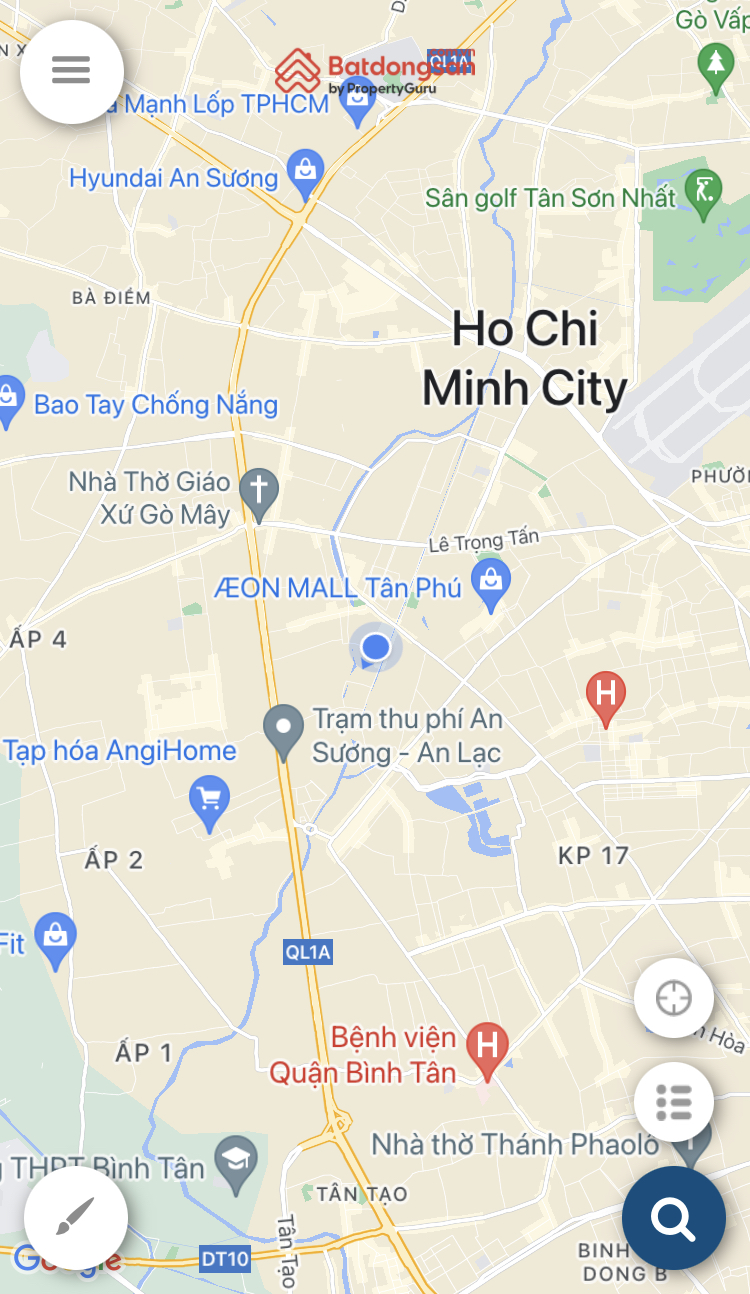
\includegraphics[width=0.5\textwidth]{Images/RelatedSystems/BatdongsanMobile.PNG}
    \caption{Giao diện Batdongsan.com.vn trên thiết bị di động}
\end{figure}
Batdongsan.com.vn là một nền tảng trực tuyến cung cấp thông tin về bất động sản, kết nối người mua, người bán, và những người quan tâm đến thị trường bất động sản. Dưới đây là một số tính năng chính của Batdongsan.com.vn:
\begin{itemize}
    \item \textbf{Tìm kiếm bất động sản}
    \begin{itemize}
    \item \textit{Tìm kiếm theo vị trí:} Người sử dụng có thể tìm kiếm bất động sản theo vị trí cụ thể, chẳng hạn như thành phố, quận, phường.
    \item \textit{Tìm kiếm theo loại bất động sản:} Tính năng này cho phép người dùng lọc kết quả theo loại bất động sản, bao gồm căn hộ, nhà riêng, đất đai, văn phòng, và nhiều loại khác.
    \item \textit{Tìm kiếm theo giá cả:} Người dùng có thể tìm kiếm bất động sản theo khoảng giá cụ thể hoặc khoảng giá ước tính.
    \item \textit{Tìm kiếm nâng cao:} Tính năng này cung cấp các tùy chọn lọc chi tiết hơn, như diện tích, số phòng ngủ, số phòng tắm, và tiện ích xung quanh.
    \end{itemize}
    \item \textbf{Đăng tải}
    \begin{itemize}
        \item \textit{Đăng tin bất động sản:} Người bán có thể đăng thông tin về bất động sản của họ, cung cấp thông tin chi tiết và hình ảnh để thu hút người mua.
        \item \textit{Quản lý tin đăng:} Tính năng này cho phép người bán quản lý và cập nhật thông tin của mình, thêm ảnh mới, chỉnh sửa mô tả, và thực hiện các thay đổi khác.
        \item \textit{Thông báo khi có người quan tâm:} Người bán có thể nhận được thông báo khi có người quan tâm hoặc liên hệ về tin đăng của họ.
    \end{itemize}
    \item \textbf{Thông tin chi tiết}
    \begin{itemize}
        \item \textit{Thông tin chi tiết về bất động sản:} Bất động sản được mô tả chi tiết với các thông tin như diện tích, hướng, tiện ích xung quanh, năm xây dựng,...
        \item \textit{Hình ảnh và video:} Người bán có thể đăng tải hình ảnh và video để người mua có cái nhìn rõ ràng về bất động sản.
        \item \textit{Liên hệ trực tiếp với người bán:} Người mua có thể liên hệ trực tiếp với người bán qua thông tin liên lạc được cung cấp trên trang tin đăng.
    \end{itemize}
    \item \textbf{Tin tức \& Phân tích}
    \begin{itemize}
        \item \textit{Tin tức:} Cung cấp các nội dung tin tức phong phú liên quan đến thị trường bất động sản để giúp người dùng có thể nắm được những thông tin nhanh và mới nhất liên quan đến lĩnh vực bất động sản
        \item \textit{Phân tích:} Những phân tích nhạy bén từ các chuyên gia kinh nghiệm trong lĩnh vực bất động sản, giúp người dùng có thể cân nhắc một cách tối ưu nhất khi đưa ra những quyết định
    \end{itemize}
    \item \textbf{Hỗ trợ}
    \begin{itemize}
        \item \textit{Trung tâm hỗ trợ:} Batdongsan.com.vn cung cấp trung tâm hỗ trợ với thông tin hữu ích và câu hỏi thường gặp để giúp người dùng.
        \item \textit{Hỗ trợ qua điện thoại và email:} Dịch vụ hỗ trợ khách hàng qua điện thoại và email để giải đáp mọi thắc mắc và giúp đỡ người dùng.
    \end{itemize}
\end{itemize}
\subsection{Phân tích SWOT}
\begin{tcbraster}[raster columns=2, boxrule=0mm, arc=0mm]
\begin{tcolorbox}[equal height group=A, size=fbox, colback=swotS!60, colframe=swotS!80!black, title=\textsc{strengths}]
\begin{itemize}
\item Batdongsan.com.vn là một trong những trang web hàng đầu về bất động sản tại Việt Nam, có lượng người dùng lớn.
\item Cung cấp thông tin đa dạng về bất động sản, từ căn hộ, nhà đất đến văn phòng, phục vụ nhu cầu đa dạng của người dùng.
\item Giao diện trực quan, dễ sử dụng, giúp người dùng dễ dàng tìm kiếm và đăng tải tin rao bán.
\item Được đầu tư bởi PropertyGuru, một trong những công ty hàng đầu về dịch vụ bất động sản châu Á, để nâng cao chất lượng dịch vụ và khả năng tiếp cận thị trường.
\end{itemize}
\end{tcolorbox}
\begin{tcolorbox}[equal height group=A, size=fbox, colback=swotW!60, colframe=swotW!80!black, title=\textsc{weaknesses}]
\begin{itemize}
\item Chất lượng thông tin về bất động sản phụ thuộc nhiều vào người đăng tin, có thể gây ra tình trạng thông tin không chính xác hoặc thiếu đầy đủ.
\item Cạnh tranh cao từ các trang web và ứng dụng bất động sản khác, đòi hỏi Batdongsan.com.vn duy trì và nâng cao chất lượng dịch vụ để giữ chân người dùng.
\item Quảng cáo có thể làm ảnh hưởng đến trải nghiệm người dùng trên trang web.
\item Một số vấn đề về pháp lý và thuế có thể phức tạp, đặt ra những thách thức cho hoạt động kinh doanh của Batdongsan.com.vn.
\end{itemize}
\end{tcolorbox}
\begin{tcolorbox}[equal height group=B, size=fbox, colback=swotO!60, colframe=swotO!80!black, title=\textsc{opportunities}]
\begin{itemize}
\item Sự phát triển nhanh chóng của thị trường bất động sản ở Việt Nam, tạo ra cơ hội cho Batdongsan.com.vn mở rộng hoạt động và tăng cường thị phần.
\item Khả năng tích hợp trí tuệ nhân tạo để cải thiện trải nghiệm người dùng và tăng tính tương tác.
\item Nhu cầu về bất động sản thông minh và hiện đại đang tăng, có thể làm tăng cơ hội cho Batdongsan.com.vn cung cấp thông tin về các dự án mới và hiện đại.
\item Hợp tác và đầu tư từ các đối tác lớn có thể giúp Batdongsan.com.vn mở rộng và cập nhật công nghệ.
\end{itemize}
\end{tcolorbox}
\begin{tcolorbox}[equal height group=B, size=fbox, colback=swotT!60, colframe=swotT!80!black, title=\textsc{threats}]
\begin{itemize}
\item Thị trường bất động sản có thể chịu ảnh hưởng lớn từ các yếu tố kinh tế và chính trị, ảnh hưởng đến nhu cầu và giá trị bất động sản.
\item Cạnh tranh cao từ các đối thủ trong và ngoài nước, có khả năng cướp khách hàng và thị phần.
\item Thay đổi trong quy định pháp lý và thuế có thể tác động đến hoạt động kinh doanh của Batdongsan.com.vn.
\item Các vấn đề về an toàn thông tin và bảo mật dữ liệu có thể ảnh hưởng đến niềm tin người dùng và hình ảnh thương hiệu.
\end{itemize}
\end{tcolorbox}
\captionof{table}{Phân tích SWOT cho Batdongsan.com.vn (PropertyGuru)}
\end{tcbraster}
\subsection{Nhận xét}
\hspace*{1cm}Batdongsan.com.vn by PropertyGuru đã đạt được vị thế lớn trong lĩnh vực bất động sản tại Việt Nam, mang lại nhiều lợi ích cho cả người mua và người bán. Nền tảng này cung cấp một nguồn thông tin đa dạng về bất động sản, giúp người mua dễ dàng tìm kiếm và so sánh. Được hỗ trợ bởi PropertyGuru, một doanh nghiệp lớn trong lĩnh vực bất động sản châu Á, đã giúp nâng cao chất lượng dịch vụ và mở rộng khả năng tiếp cận thị trường.\\
\hspace*{1cm}Giao diện trực quan và dễ sử dụng của Batdongsan.com.vn cũng là một điểm mạnh, tạo ra trải nghiệm người dùng tích cực. Việc cung cấp thông tin đầy đủ và chính xác về bất động sản giúp người mua có quyết định đúng đắn khi lựa chọn chỗ ở. Hơn nữa, cơ hội để đầu tư và phát triển trong ngành bất động sản đang ngày càng mở rộng.\\
\hspace*{1cm}Tuy nhiên, để duy trì vị thế của mình, Batdongsan.com.vn cũng phải đối mặt với một số thách thức. Cạnh tranh cao từ các đối thủ trong và ngoài nước đặt ra áp lực để duy trì và nâng cao chất lượng dịch vụ. Ngoài ra, các vấn đề pháp lý và thuế cũng có thể tác động đến hoạt động kinh doanh của họ. Điều này đòi hỏi sự quan tâm và linh hoạt trong quản lý để đối mặt với những thách thức này và tiếp tục phát triển một cách bền vững.